\chapter[Detección de vegetación flotante en el RdP]{Detección y cuantificación de vegetación flotante en aguas turbias del Río de la Plata utilizando imágenes ópticas de alta resolución}
\label{cam} 

El desarrollo masivo de plantas flotantes en lagos de llanuras y humedales en el río Paraná medio superior en la Cuenca del Plata tiene un apreciable impacto tanto ambiental como socioeconómico. Cada año, los desprendimientos de plantas acuáticas se desplazan río abajo llegando en pequeñas cantidades al RdP, pero se han observado grandes invasiones temporarias cada 10 ó 15 años asociadas a inundaciones masivas. Desde finales de diciembre de 2015 las fuertes lluvias, muy probablemente provocadas por una fase positiva de El Niño, aumentaron los niveles de los ríos tributarios al RdP provocando una gran invasión temporaria de plantas acuáticas de enero a mayo de 2016. Este evento causó una interrupción significativa de las actividades humanas debido a la obstrucción de las tomas de agua potable en el estuario, bloqueando puertos y marinas e introduciendo animales peligrosos de humedales lejanos en la ciudad de Buenos Aires.

En este capítulo se presenta un esquema que ha sido desarrollado para detectar y mapear la vegetación flotante en aguas turbias utilizando imágenes de alta resolución, como Sentinel-2/MSI, Landsat-8/OLI y Aqua/MODIS-250m. Para su diseño fue utilizada una combinación del índice de algas flotantes FAI (\textit{Floating Algal Index}, que utiliza la fuerte señal en el NIR), además de umbrales establecidos para la banda roja (para evitar clasificar erróneamente las aguas altamente turbias) y en las coordenadas del espacio de color CIE-La$^{*}$b$^{*}$ (para confirmar los píxeles visualmente \textit{verdes} como vegetación flotante). Se analizó una serie temporal de imágenes de alta resolución multisensor para estudiar la variabilidad temporal, el área cubierta y la distribución de la inusual invasión de plantas vasculares acuáticas flotantes ocurrida en enero de 2016 en el RdP.

$\quad$

\noindent
El contenido del presente capítulo se halla publicado en

$\quad$

\noindent
DOGLIOTTI, ANA I., GOSSN, JUAN I., VANHELLEMONT, QUINTEN, RUDDICK, KEVIN G. (2018) Detecting and Quantifying a Massive Invasion of Floating Aquatic Plants in the Río de la Plata Turbid Waters Using High Spatial Resolution Ocean Color Imagery, Remote Sensing, 2072-4292 10(7) 1140 doi:10.3390/rs10071140 https://www.mdpi.com/ 2072-4292/10/7/1140, \cite{dogliotti2018}

\section{Introducción}
\label{cam:s:introduccion}

    El jacinto de agua (\textit{Eichhornia crassipes}) es una planta macrófita autóctona de la Baja Amazonia, Brasil, que forma densas matas en la superficie de las vías fluviales y las aguas estancadas. En los humedales de llanuras aluviales, las plantas vasculares acuáticas desempeñan un papel crucial, ya que participan en los ciclos de vida de varias otras especies que proporcionan alimento, sitios de anidación, refugio, etc., y también pueden interactuar con otros factores que modifican algunas características físicas y químicas del medio ambiente, como la transparencia del agua, las tasas de sedimentación, etc. \cite{marchetti2013}. Por otro lado, la proliferación masiva del jacinto de agua podría representar una amenaza significativa para la recreación, la pesca, los recursos de vida silvestre y los procesos ecológicos de los ecosistemas de agua dulce, como ha ocurrido en el lago Victoria en África Oriental \cite{fusilli2013}, el Río Grande \cite{everitt2003} y en el delta del Río Sacramento-San Joaquín de California en los Estados Unidos \cite{cohen1998}.
    
    El mapeo de plantas acuáticas y la estimación de su extensión superficial son cruciales para el manejo eficiente y la implementación de medidas de mitigación. Esta información se puede derivar con precisión con productos de teledetección de alta resolución, como las imágenes proporcionadas por los sistemas Sentinel-2/MSI (10 m) y Landsat-8/OLI (30 m), pero su baja frecuencia de observación y  estrecha franja de barrido (\textit{swath}) dificultan su capacidad de monitorear y cuantificar continuamente la extensión de la vegetación flotante. Por otro lado, los sensores de resolución media, como MODIS (250 m), OLCI (300 m) y PROBA-V (100 m) proporcionan una vista más amplia y con mayor frecuencia de datos, pero a expensas de los detalles espaciales. Existen diferentes índices que permiten detectar la vegetación acuática flotante utilizando datos de teledetección que hacen uso de su fuerte reflectancia en el infrarrojo cercano (NIR), similar a la de la vegetación terrestre \cite{gower2008}\cite{hu2009}\cite{shi2009}\cite{keesing2011}\cite{alawadi2010}\cite{xing2016}\cite{hu2017}. Estos índices han sido originalmente diseñados para aguas claras, pero su aplicabilidad en aguas turbias no es sencilla, como mencionaron Hu et al. 2015 \cite{hu2015} y como fue analizado por Liang et al. 2017 \cite{liang2017}.
    
    En la llanura de inundación del río Paraná (Argentina) (Figura \ref{cam:parana}) la vegetación acuática flotante representa una biomasa importante - movilizada por pulsos de inundación y factores climáticos - y su deriva mueve materia orgánica, insectos y otros organismos en el sistema ecológico. Los desprendimientos de plantas acuáticas derivan río abajo llegando en pequeñas cantidades al RdP cada año, pero se han observado invasiones más masivas cada 10 ó 15 años. A mediados de enero de 2016, la costa de Buenos Aires se cubrió con grandes matas de jacinto acuático \textit{Eichhornia crassipes}. Este evento extraordinario se relacionó con lluvias inusualmente fuertes que ocurrieron en el sur de Sudamérica a fines de 2015 - asociadas con un fuerte fenómeno de El Niño, \cite{ropewelski1987}\cite{mason2001} - que inundó los ríos tributarios al RdP. La lluvia y las inundaciones elevaron los niveles de agua de las llanuras aluviales a lo largo del río Paraná y barrieron las plantas flotantes hacia la vía fluvial principal (Figura \ref{cam:parana}b). Esta invasión masiva temporaria de plantas acuáticas que ocurrió de enero a fines de abril de 2016 causó una interrupción significativa de las actividades humanas a causa de la obstrucción de las tomas de agua potable en el estuario, el bloqueo de puertos comerciales y deportivos y la introducción de animales peligrosos pertenecientes a humedales lejanos a la ciudad de Buenos Aires.
    
    El objetivo del presente estudio es evaluar la invasión inusual de \textit{Eichhornia crassipes} ocurrida en el RdP desde una perspectiva de múltiples misiones. Se desarrolla una metodología utilizando un conjunto de índices y condiciones para detectar la presencia del jacinto de agua en las aguas turbias del RdP utilizando imágenes de Sentinel-2A/MSI, Landsat-8/OLI y Aqua/MODIS-250m; se discute el impacto de diferentes resoluciones espaciales en la detección de la vegetación flotante (VF), y finalmente se analiza y cuantifica su extensión espacial y variabilidad temporal y su relación con el caudal de salida del río.
    
    
    \begin{figure}
    \centering
    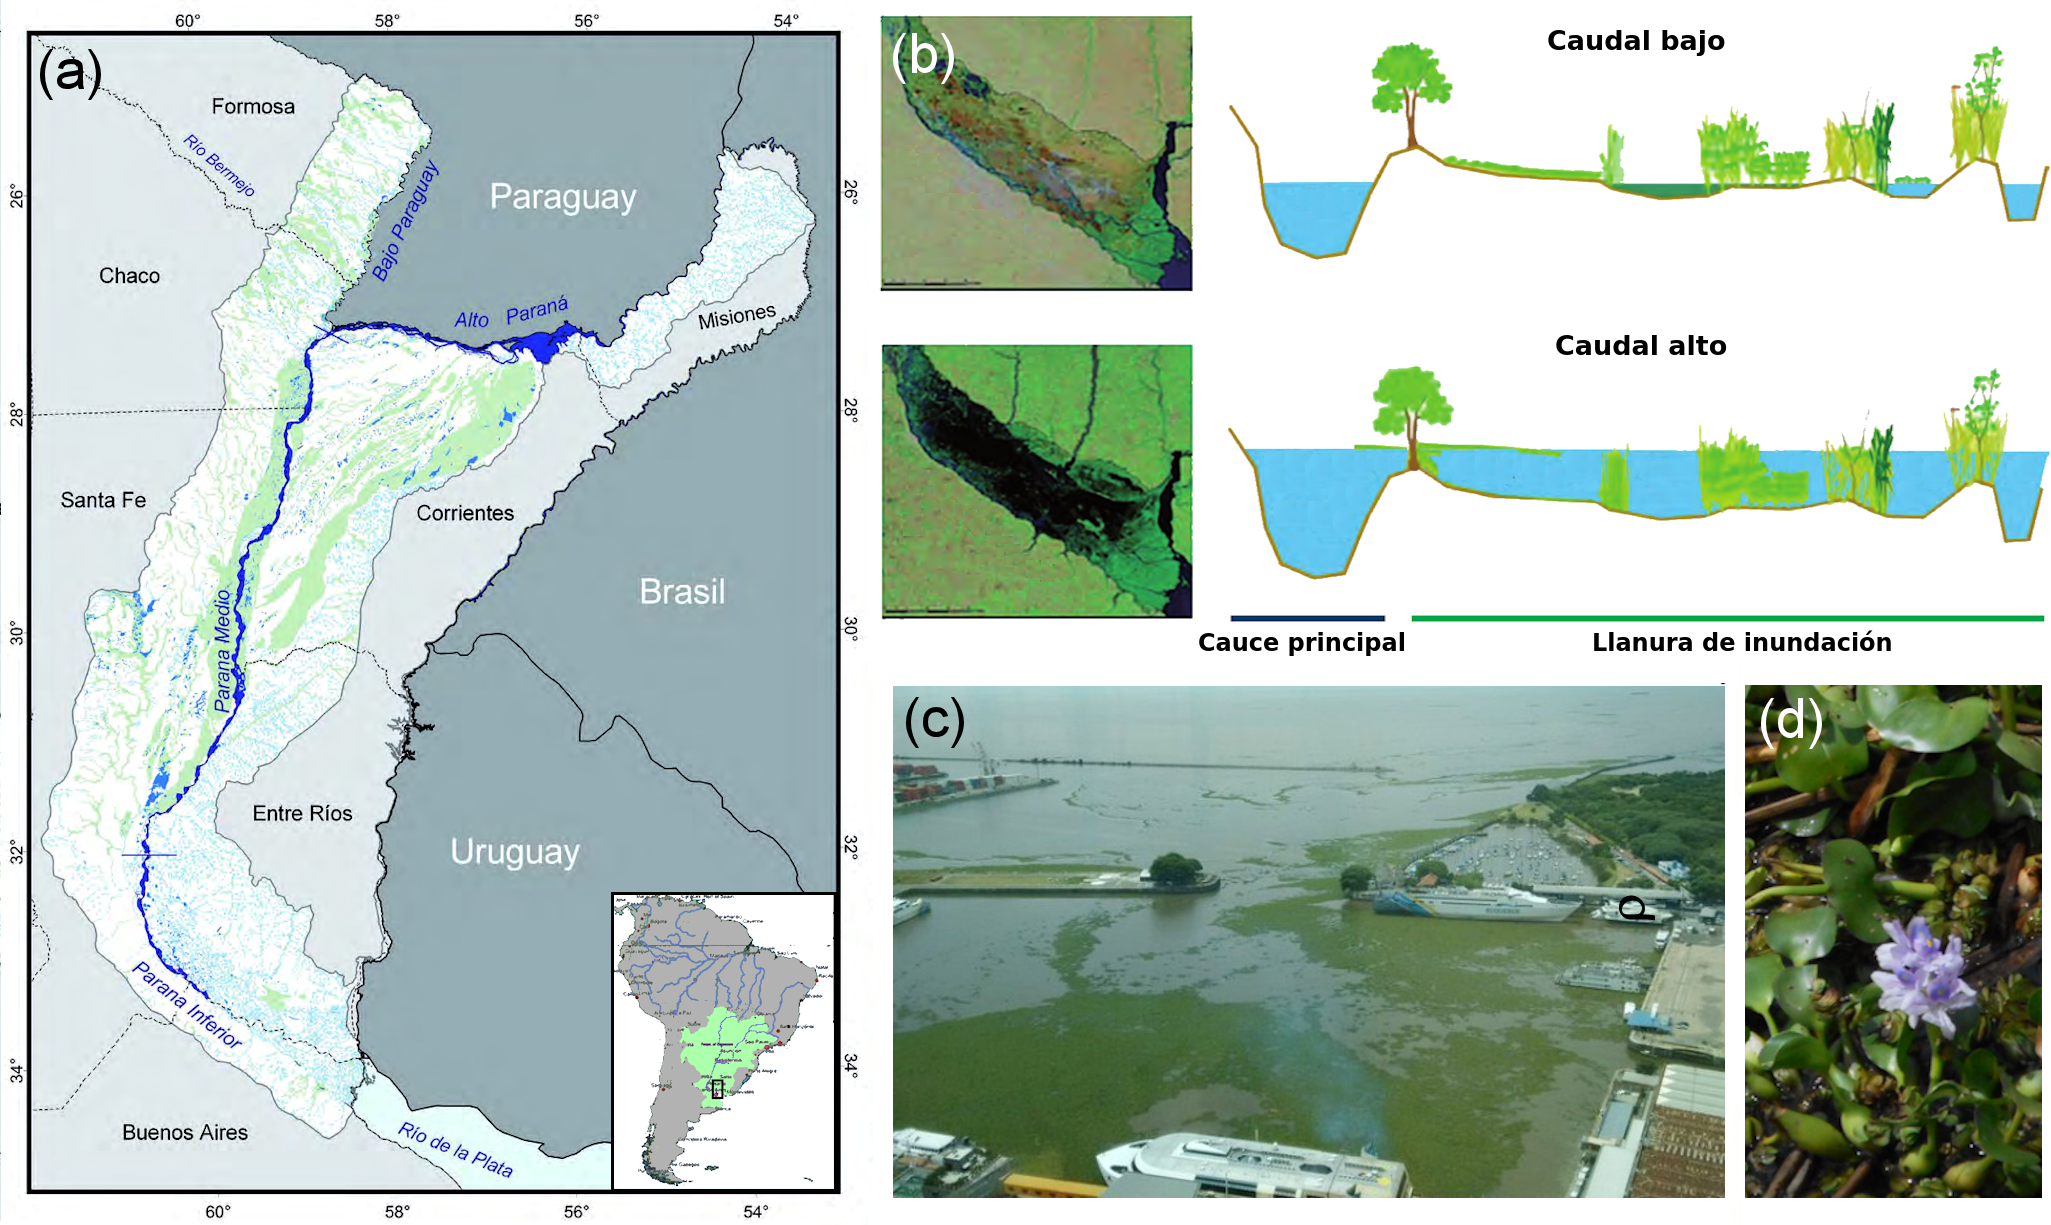
\includegraphics[width=\textwidth]{cam/figures/parana.png}
    \caption[Ubicación del corredor fluvial de los ríos Paraná, Paraguay y RdP y representación esquemática de niveles de agua bajo y alto]{(a) Ubicación del corredor fluvial de los ríos Paraná y Paraguay y el Estuario del RdP; (b) representación esquemática de niveles de agua bajo y alto, junto con composiciones RGB de Landsat, donde los píxeles con agua se ven en azul oscuro (modificado de \cite{minotti2013}); c) Una terminal de ferris invadida por jacinto de agua (d).}
    \label{cam:parana}
    \end{figure}

\section{Materiales y métodos}
\label{cam:s:materiales}

    \subsection{Datos satelitales}
    \label{cam:s:datasat}
        
        Diversos datos satelitales con diferentes resoluciones espaciales y temporales que cubren la región RdP en el período 2015-2016 se utilizaron en el presente estudio (Cuadro \ref{cam:tab:sistemas}). Las imágenes Aqua/MODIS (MA) L1A se descargaron del sitio web de NASA Ocean Color (http://oceancolor.gsfc.nasa.gov); las imágenes LandSat-8/OLI (L8) L1T ortorrectificadas y corregidas por el terreno se descargaron de USGS EarthExplorer (\url{http://earthexplorer.usgs.gov}) y las imágenes Sentinel-2A/MSI (S2A) L1C de ESA Copernicus Open Access Hub (\url{https://scihub.copernicus.eu}).

        La reflectancia corregida por Rayleigh ($\rho_{RC}$) en todas las bandas se obtuvo utilizando diferentes programas disponibles para los diferentes sensores: los datos MODIS se procesaron con SeaDAS v7.4, y los datos OLI y MSI se procesaron con el software ACOLITE (Atmospheric Correction for OLI \textit{lite}) v.20170718.1 \cite{vanhellemont2014}\cite{vanhellemont2015}. También se generaron imágenes RGB de color cuasi verdadero para cada sensor utilizando las bandas roja (R), verde (G) y azul (B) correspondientes a cada sensor (ver Cuadro \ref{cam:tab:sistemas}). Las imágenes diarias de Aqua/MODIS se mapearon en una proyección equidistante cilíndrica a una resolución espacial de $0.002\degree$ ($\sim 250$ m).


        \begin{table}
        \tiny
        \setlength\tabcolsep{1.5pt} % default value: 6pt
        \caption[Lista de los sistemas satelitales utilizados para la detección de vegetación flotante.]{Lista de los sistemas satelitales utilizados en este capítulo. Tiempos de revisita, anchos de la franja de barrido (\textit{swaths}), resoluciones espaciales y longitudes de onda centrales (en nm) y anchos de banda (entre paréntesis) de las bandas utilizadas para identificar vegetación flotante.}
        \begin{tabular}{|c|c|c|c|c|c|c|c|c|}
        \hline
        \textbf{Sensor} & \textbf{Revisita} & \textbf{Swath km]}      & \textbf{Resolución [m]} & \textbf{Rojo [nm]} & \textbf{Verde [nm]} & \textbf{Azul [nm]} & \textbf{NIR [nm]} & \textbf{SWIR [nm]} \\ \hline
        \multirow{2}{*}{\textbf{Aqua/MODIS}} & \multirow{2}{*}{Diaria}   & \multirow{2}{*}{2330} & 250     & 645 (50)  &     &    & 859 (250) &    \\ \cline{4-9} 
             &          &       & 500     &   & 555 (20)    & 469 (20)   &   & 1240 (20)  \\ \hline
        \textbf{L8/OLI}      & 8 ó 16 días     & 180   & 30      & 655 (50)  & 561 (75)    & 483 (65)   & 865 (40)  & 1650 (100) \\ \hline
        \multirow{2}{*}{\textbf{S2A/MSI}}    & \multirow{2}{*}{10 días} & \multirow{2}{*}{290}  & 10      & 665 (30)  & 560 (35)    & 497 (65)   &   &    \\ \cline{4-9} 
             &          &       & 20      &   &     &    & 865 (20)  & 1610 (90)  \\ \hline
        \end{tabular}
        \label{cam:tab:sistemas}
        \end{table}

    \subsection{Datos de campo}
    \label{cam:s:data}
        Se realizaron mediciones de reflectancia de una mata densa de jacinto acuático el 28 de enero de 2016, desde un muelle ubicado en la ciudad de Tigre, al norte de la ciudad de Buenos Aires y cerca del Delta del Paraná. Se montaron dos espectrorradiómetros hiperespectrales Trios-RAMSES, que miden la radiancia ascendente y la irradiancia descendente siguiendo el protocolo descrito en \S \ref{dat:s:triosMed}. La única modificación respecto de dicho protocolo es que no se realizó ninguna corrección para la reflexión de la interfase aire-agua de la radiación del cielo porque la mayor parte de la superficie estaba cubierta por vegetación - es decir, se consideró $\rho_{sky}=0$.
        %
        En la Figura \ref{cam:firmaCamalote}, la reflectancia espectral medida del jacinto acuático se compara con los espectros de reflectancia de agua previamente adquridos entre 2012 y 2016 durante varias campañas y en diferentes regiones del RdP.

\section{Resultados y discusión}
\label{cam:s:resultados}

    \subsection{Características espectrales de la especie \textit{Eichhornia crassipes}}
    \label{cam:s:eichhornia}

        La reflectancia de los entramados de \textit{Eichhornia crassipes} se recolectó cerca de la ciudad de Buenos Aires durante la invasión de vegetación flotante en enero de 2016 (Figura \ref{cam:firmaCamalote}). Los espectros mostraron características espectrales típicas de las plantas vasculares acuáticas flotantes, es decir, un marcado aumento de la reflectancia en el NIR (700-900 nm), principalmente debido a la estructura celular de las hojas en el caso específico de \textit{E. crassipes}, y un pico en la región verde ($\sim 550$ nm) debido a la absorción de clorofila-a en las partes azul y roja (675 nm) del espectro (espectros verdes en la Figura \ref{cam:firmaCamalote}). Este aumento de la reflectancia en el NIR, conocido como reflectancia del borde rojo (\textit{red edge}), también puede ser causado por otros organismos o materiales que flotan en la superficie, como pastos marinos (\textit{seagrass}) y la acumulación de células de cianobacterias en la superficie que forman una espuma densa y que reducen el efecto absorbente del agua. Las nueve mediciones realizadas apuntando el radiómetro en ángulos de azimut ligeramente diferentes cerca de $135\degree$ mostraron una mayor variabilidad en la región NIR (líneas verdes discontinuas). Esto probablemente se deba al diferente porcentaje de área cubierta por vegetación y agua dada la naturaleza no homogénea y móvil del objetivo (Figura \ref{cam:firmaCamalote}), así como la posible dependencia direccional (azimutal) para la reflectancia de la vegetación. Para la comparación se muestran en negro en la Figura \ref{cam:firmaCamalote} los espectros medios (línea sólida gruesa) y más/menos un desvío estándar (líneas discontinuas) de más de 50 mediciones de campo recolectadas en las aguas turbias del RdP. Los espectros medios de las aguas turbias muestran características típicas que son esperadas en el estuario superior (cerca de Buenos Aires), tales como las descritas en \S \ref{dat:s:radiometricas} (ver Figuras \ref{dat:HyperASD} y \ref{dat:HyperTriOS}).


        \begin{figure}
        \centering
        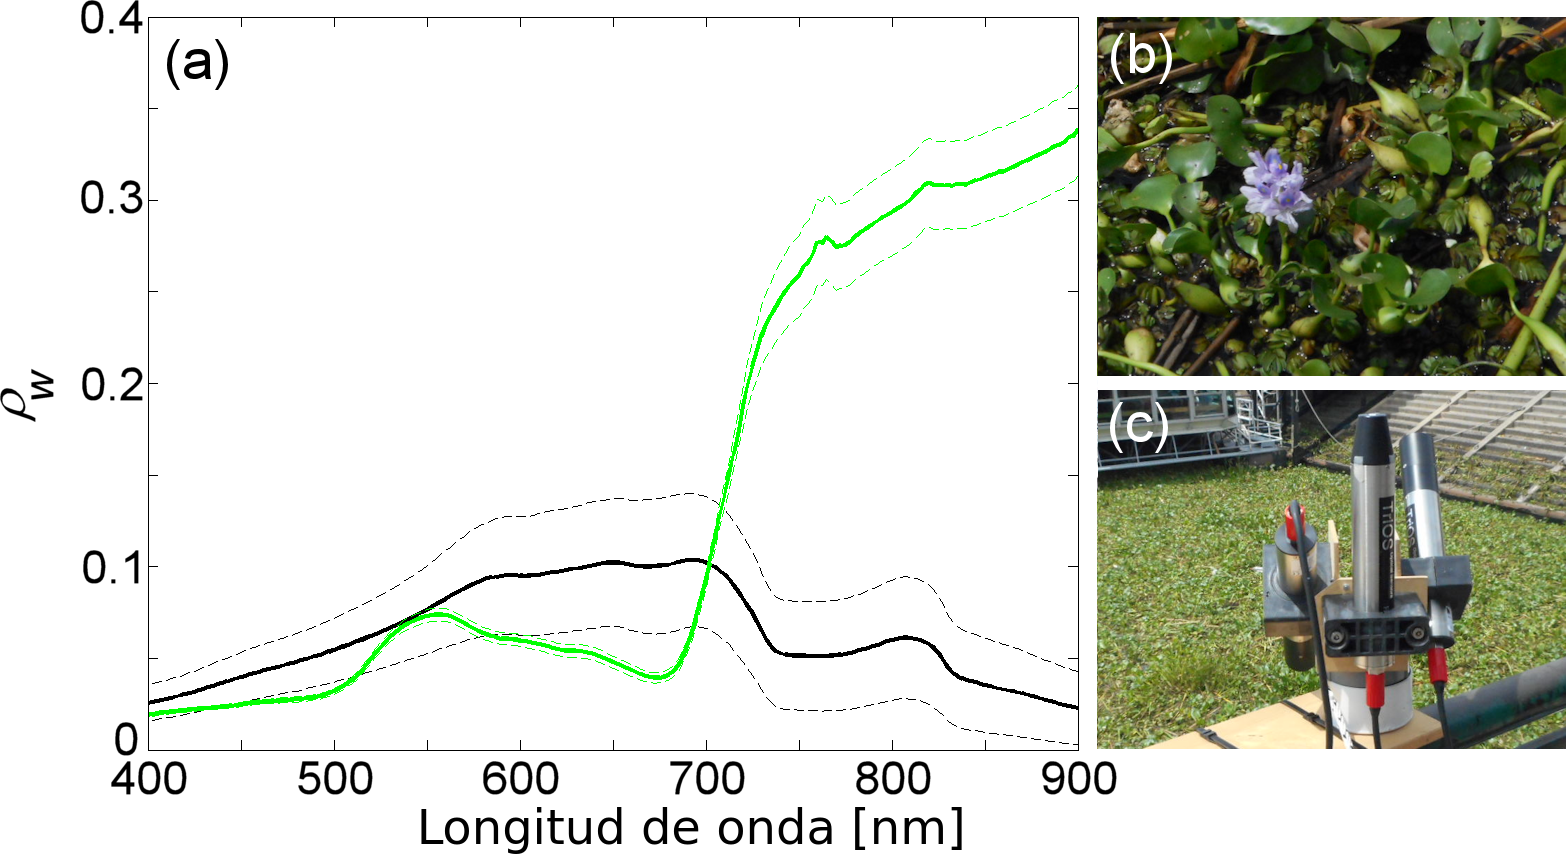
\includegraphics[width=0.8\textwidth]{cam/figures/firmaCamalote.png}
        \caption[Reflectancias \textit{in situ} de matas de jacinto de agua y de aguas turbias del RdP]{(a) Reflectancias \textit{in situ} de matas de jacinto de agua (verdes) recolectadas en enero de 2016 y aguas turbias del RdP (negras) colectadas en campañas anteriores. Las líneas gruesas representan la media de 9 mediciones de \textit{Eichhornia crassipes} y >50 mediciones de aguas turbias del RdP, respectivamente. Las líneas discontinuas corresponden a un desvío estándar. (b) Fotografías de jacinto de agua flotante \textit{E. crassipes}, y (c) configuración de medición.}
        \label{cam:firmaCamalote}
        \end{figure}

    
    \subsection{Identificación de vegetación flotante}
    \label{cam:s:identificacion}
    
        La detección de VF usando la teledetección se ha realizado generalmente utilizando índices que hacen uso de su fuerte señal en el NIR y el SWIR, que es similar al de la vegetación terrestre y contrasta altamente con la baja señal proveniente del agua. Un ejemplo es el Índice de Vegetación de Diferencia Normalizada (NDVI). Para detectar \textit{E. crassipes} en las aguas altamente turbias del RdP, se ha utilizado una combinación de diferentes índices y umbrales que se describen en esta sección.

        El índice de algas flotantes (FAI), que se ha utilizado para detectar algas flotantes debido a la elevada reflectancia en el NIR \cite{hu2010b}, se define, siguiendo la notación del capítulo \ref{blr} como

        \begin{equation}
            FAI = BLR(\rho_{RC})[\lambda_{Rojo},\lambda_{NIR},\lambda_{SWIR}]
            \label{cam:eq:fai}
        \end{equation}
        
        \noindent
        donde $\lambda_{x}$ es la longitud de onda central de cada banda $x=Rojo, NIR, SWIR$ correspondiente al sensor (Cuadro \ref{cam:tab:sistemas}). En general, los valores positivos de FAI indican la presencia de vegetación fuera del agua.

        \begin{figure}
        \centering
        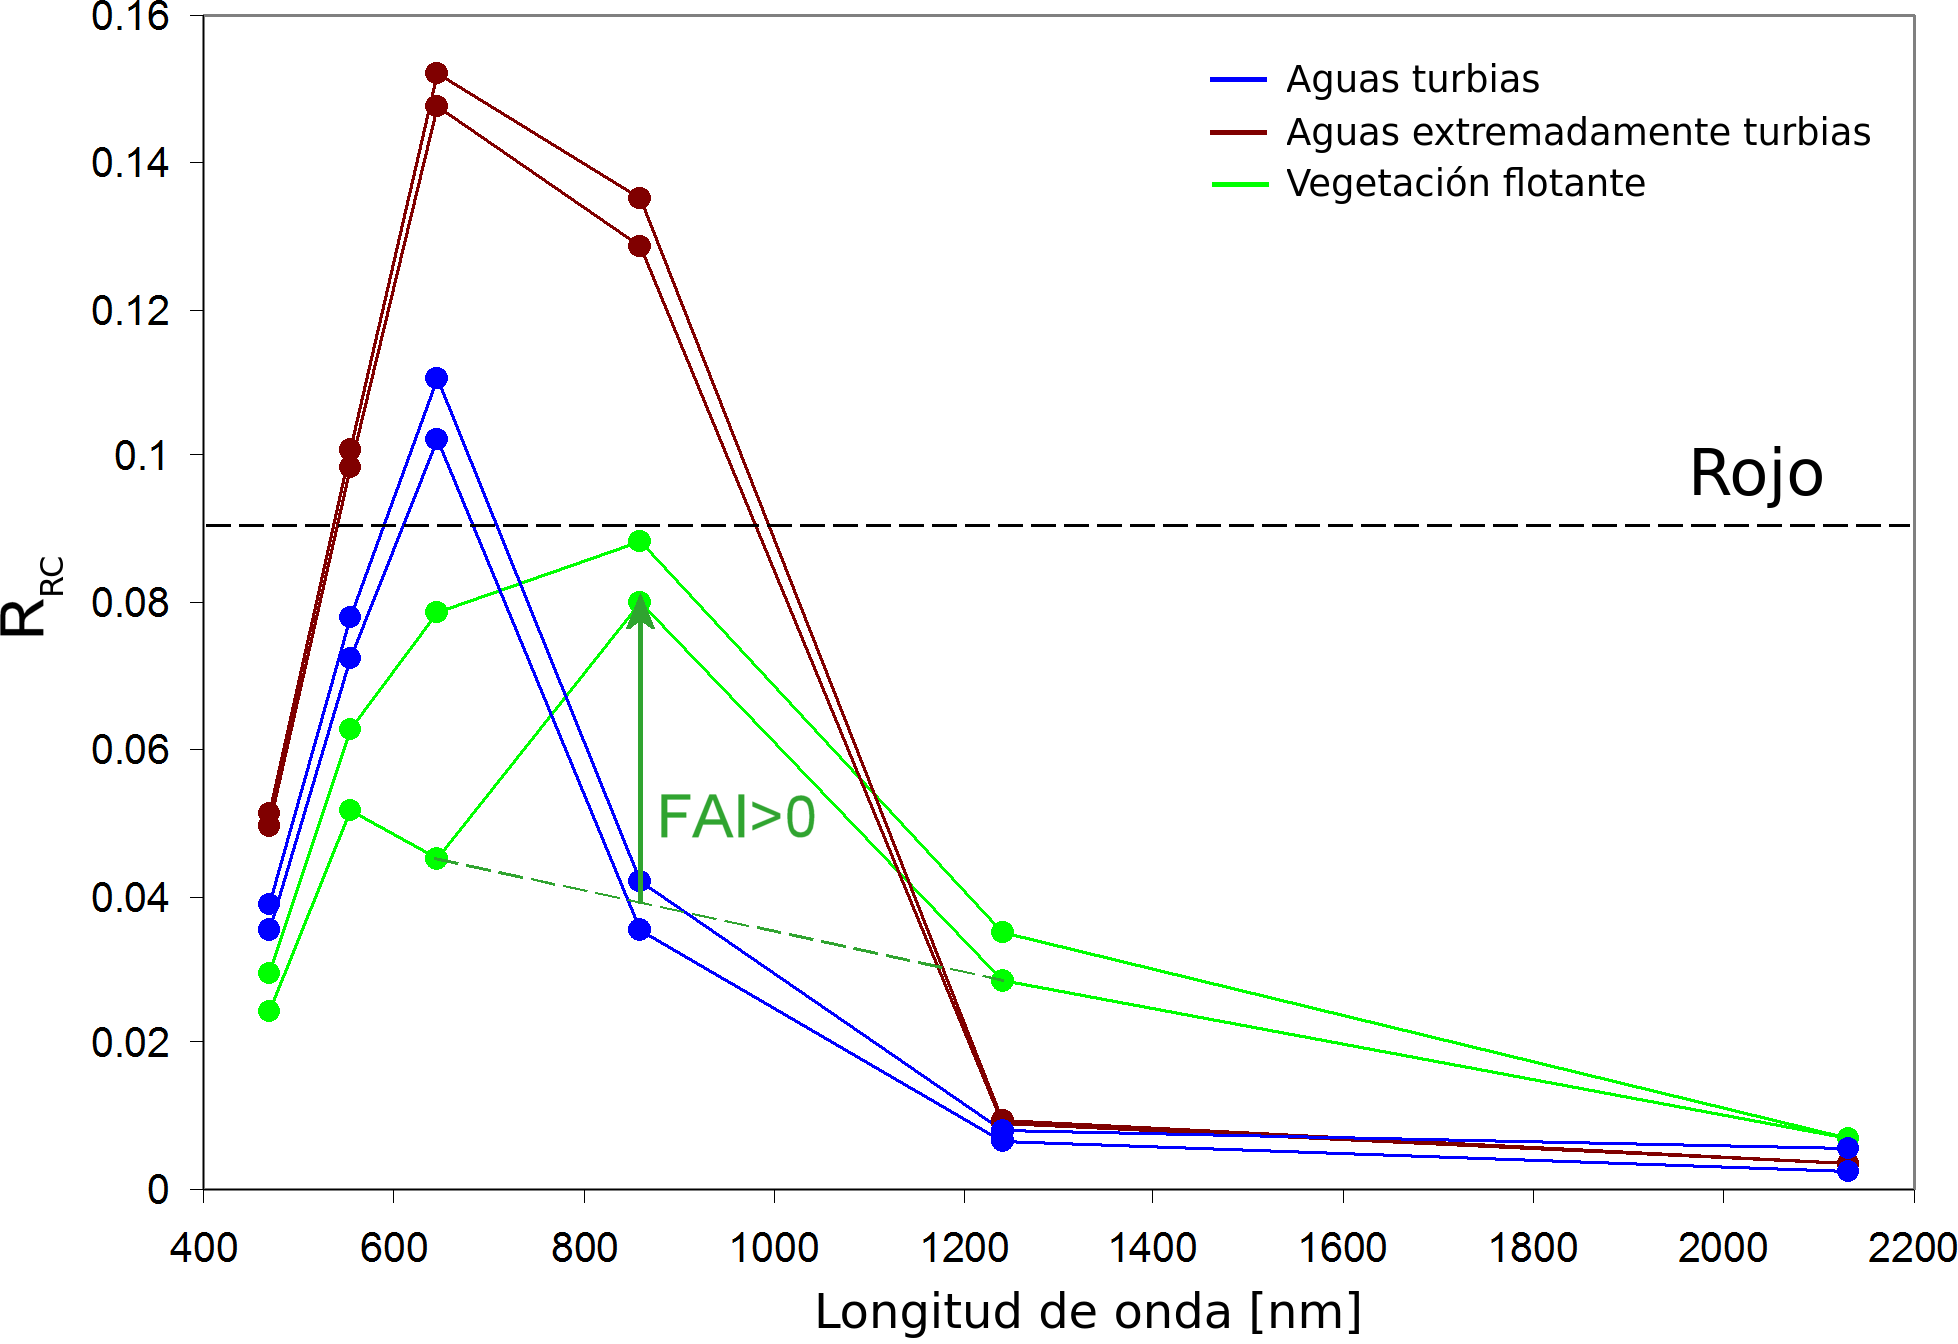
\includegraphics[width=0.8\textwidth]{cam/figures/firmasFAI.png}
        \caption[Espectros de píxeles corregidos por Rayleigh con vegetación flotante, correspondientes a aguas turbias y a aguas turbias extremas.]{Espectros de píxeles corregidos por Rayleigh i) que se ven verdes en la combinación RGB - por lo que contienen una cantidad detectable de vegetación flotante - (en verde), ii) correspondientes a aguas turbias (en azul), y iii) correspondientes a aguas turbias extremas (en marrón), extraídos de una imagen Aqua/MODIS del RdP. El índice FAI se indica esquemáticamente, así como el umbral aplicado a la reflectancia corregida por Rayleigh $\rho_{RC}$ en la banda roja.}
        \label{cam:firmasFAI}
        \end{figure}

        En la zona de máxima turbidez del RdP (Barra del Indio, Figura \ref{int:rdp}), la reflectancia es muy alta en el NIR (alta concentración de partículas) y más baja en las bandas roja y SWIR (alta absorción de agua), lo que da un pico en el NIR que se interpreta erróneamente como un píxel con VF por el FAI (espectros marrones en Figura \ref{cam:firmasFAI}). Para evitar estos falsos positivos en las aguas más turbias, se determinó un umbral en la banda roja. En aguas de baja y moderada turbidez,  sería útil utlizar un umbral en la banda SWIR, pero debido a la contribución de los aerosoles, el \textit{sunglint} y la gran cantidad de sedimentos que afectan la banda MODIS de 1240 nm \cite{shi2009}, se han encontrado valores de reflectancias RC similares para aguas muy turbias y VF.
        A su vez, la banda roja se ve afectada por la absorción de la clorofila-a presente en la VF (implicando una disminución en la reflectancia) y por la dispersión de partículas (implicando un aumento de la reflectancia). El umbral se definió mediante el análisis de una serie temporal de imágenes de 2 años sobre la región de mayor turbidez, siguiendo lo propuesto por Liang et al. 2017 \cite{liang2017}. Por lo tanto, se estableció un umbral de 0.08 en la reflectancia corregida por Rayleigh en la banda del rojo para diferenciar los píxeles de agua altamente turbias de los píxeles con vegetación.
        
        Se establecieron criterios adicionales para diferenciar la VF de otros objetivos que claramente no eran vegetación mediante inspección visual de las composiciones RGB, como barcos, regiones de acumulación de sedimentos por encima de la superficie y bordes de nubes. Dado que la inspección visual es la única forma de validar los resultados, se utilizaron las métricas del espacio de color CIE 1976 Lab (de ahora en adelante, La$^{*}$b$^{*}$) \cite{cie2016} para cuantificar las diferencias de color según la percepción humana. La$^{*}$b$^{*}$ es un espacio tridimensional, isomorfo a RGB, descrito por las variables de color L, a$^{*}$ y b$^{*}$. Básicamente, L representa la luminosidad y toma valores de 0 (negro absoluto) a 100 (blanco absoluto), mientras que a$^{*}$ esencialmente separa el verde (a$^{*}$<0) del rojo (a$^{*}$> 0), y b$^{*}$ separa el azul (b$^{*}$<0) de amarillo (b$^{*}$>0). El isomorfismo que lo define desde el espacio de color RGB es una transformación no lineal y se describe en detalle en \cite{cie2016}. Las variables La$^{*}$b$^{*}$ se calcularon aplicando la función \textit{color.rgb2lab} del módulo de Python \textit{skimage} a la matriz RGB definida como una combinación de reflectancias RC en las bandas roja, verde y azul (Cuadro \ref{cam:tab:sistemas}), normalizado a un umbral máximo de 0.12 para mejorar el contraste de color en ausencia de nubes. Dado que los píxeles de VF se pueden identificar por su color verdoso, se estableció una condición en el límite superior de a$^{*}$. Los umbrales en a$^{*}$ se determinaron empíricamente mediante inspección visual para cada sensor: 0 para S2, 5 para L8 y 10 para MA. Esta condición ayuda a excluir objetivos como barcos y la acumulación de sedimentos fuera de la superficie y algunos píxeles en el borde de nubes, principalmente en imágenes de alta resolución como L8 y S2A (Figura \ref{cam:embarcacion}). Se aplicaron diferentes umbrales a$^{*}$ a diferentes sensores, principalmente porque i) las composiciones RGB se definen utilizando tripletes de bandas que poseen características espectrales diferentes, lo que significa una apariencia de color diferente para cada sensor, y ii) diferentes resoluciones pueden producir diferentes firmas de color según el área cubierta (ver la siguiente sección). Para evitar más falsos positivos, generalmente ubicados en píxeles del borde de la nube con características espectrales muy variables y color aparente, las mismas se enmascararon cuando L = 100 y la máscara se extendió espacialmente por un número determinado de píxeles que variaron para cada sensor (10, 5 y 6 píxeles para S2A, L8 y MA, respectivamente). Obsérvese que la condición de L = 100 es equivalente a la condición min(R, G, B)> 0.12, ya que 0.12 fue el factor de normalización aplicado a todas las composiciones RGB.


        \begin{figure}
        \centering
        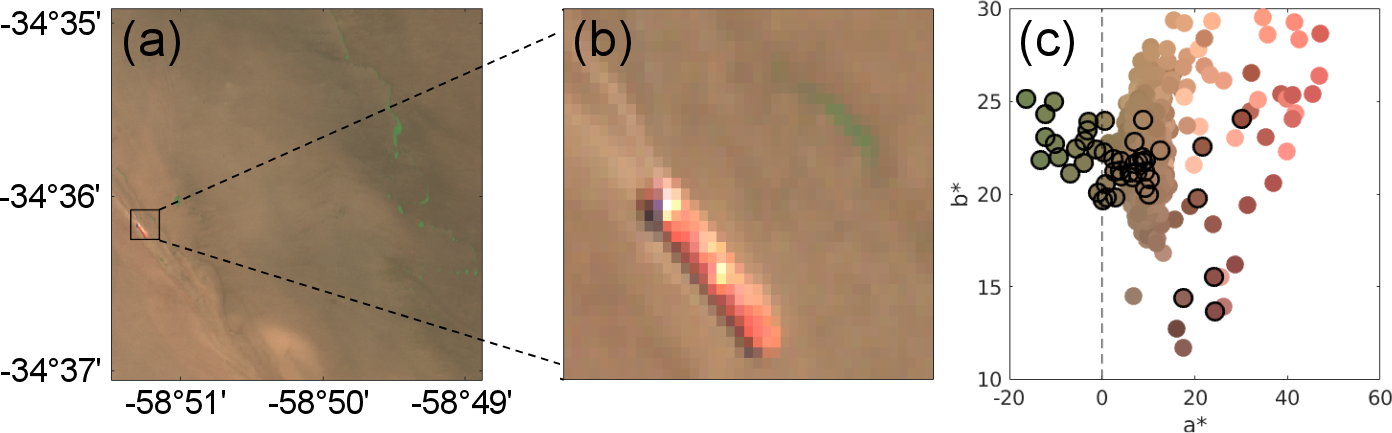
\includegraphics[width=\textwidth]{cam/figures/embarcacion.png}
        \caption[Imagen S2 mostrando un área con vegetación flotante y con una embarcación y diagrama a$^{*}$ vs b$^{*}$ de los píxeles de la imagen]{(a) Subconjunto de imagen S2 (9 de febrero de 2016) y (b) ampliación de un área con VF y con una embarcación; (c) diagrama a$^{*}$ vs b$^{*}$ de los píxeles en b) coloreados con los valores RGB. Los píxeles que pasaron los primeros criterios espectrales (FAI> 0 y Rojo> 0.09) se indican con un contorno negro, mientras que la línea discontinua indica el umbral a$^{*}$ utilizado para diferenciar la VF de embarcaciones y otros objetos flotantes.}
        \label{cam:embarcacion}
        \end{figure}
        
    \subsection{Método de clasificación aplicado en el RdP}
    \label{cam:s:clasificacion}
    
        En un primer análisis, se evaluó la capacidad de los índices NDVI \cite{shi2009} y FAI para detectar la invasión de jacintos acuáticos en el RdP \cite{dogliotti2016b}. De manera similar a los resultados de Hu, 2009 \cite{hu2009}, encontramos que el NDVI identifica sistemáticamente como VF menos píxeles en comparación con el FAI y un análisis visual indicó que el NDVI era más conservador mientras que el FAI identificaba los píxeles que un observador identificaría como \textit{verdosos} o píxeles que contienen vegetación (Figura \ref{cam:FAIvsNDVI}). Esto y el hecho de que el FAI se ve menos afectado que el NDVI por los efectos atmosféricos como los aerosoles y las condiciones de observación (descrito en detalle en el capítulo \ref{blr}, \cite{hu2009}), llevó a la selección del FAI para su uso en el presente estudio.


        \begin{figure}
        \centering
        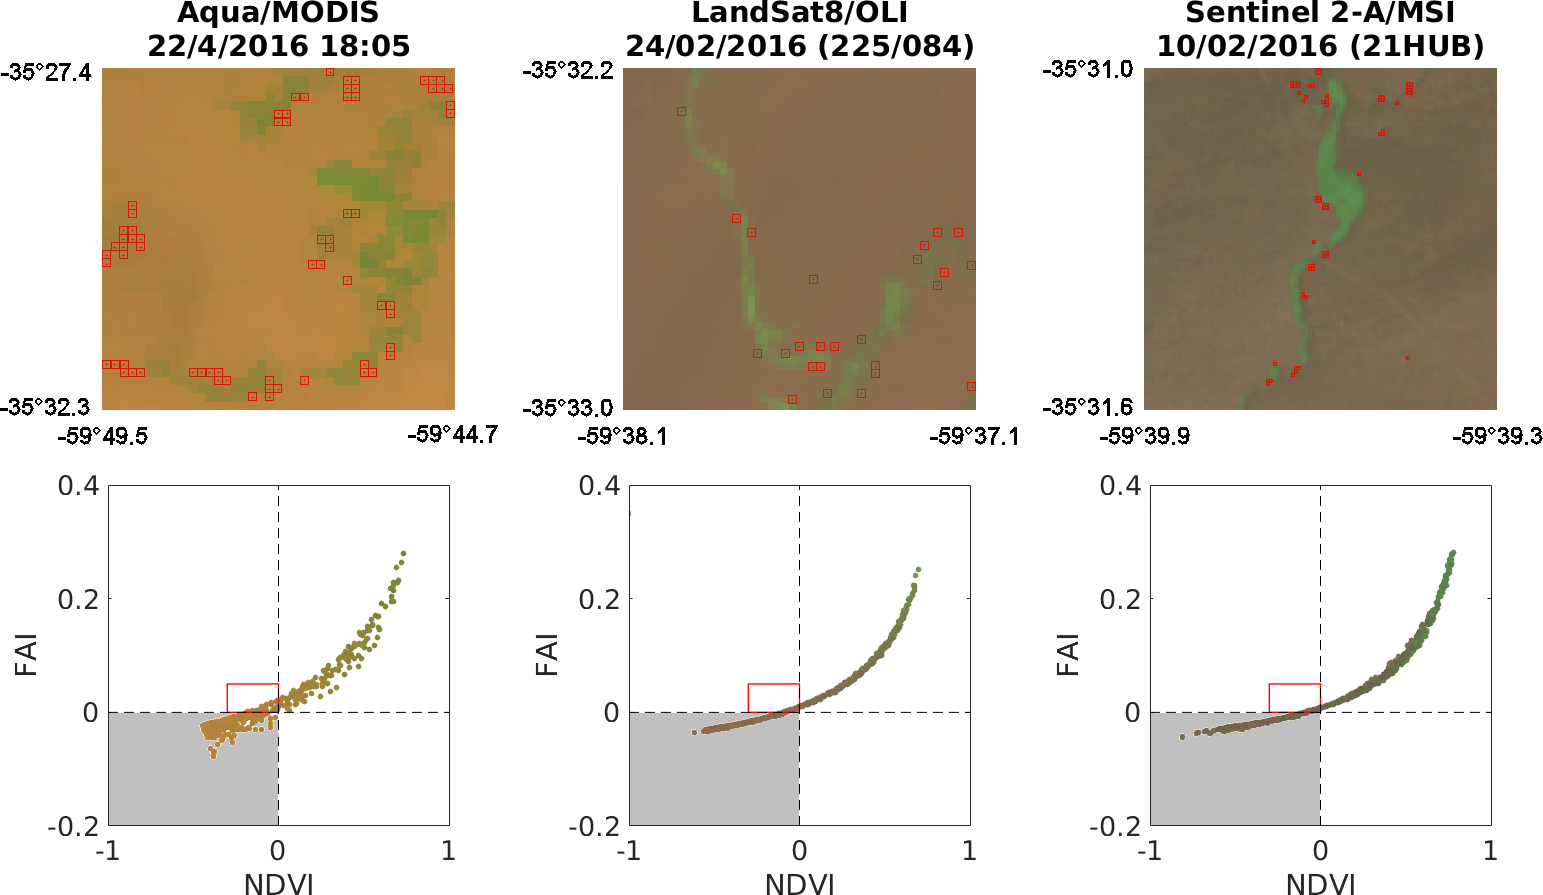
\includegraphics[width=\textwidth]{cam/figures/FAIvsNDVI.png}
        \caption[Composiciones RGB de los entramados de VF para los sistemas Aqua/MODIS, OLI y MSI-A en diferentes fechas, indicando los píxeles marcados como vegetación flotante por FAI pero no por NDVI.]{Fila superior: composiciones RGB de los entramados de VF para los sistemas Aqua/MODIS, LandSat8/OLI y Sentinel-2A/MSI en diferentes fechas. Los cuadrados rojos indican los píxeles marcados como VF por FAI pero no por NDVI. Fila inferior: FAI vs. NDVI para cada imagen, también indicados los píxeles marcados como VF por FAI pero no por NDVI por el área del cuadrado rojo. El área gris corresponde a los píxeles no identificados como VF ni por FAI ni NDVI.}
        \label{cam:FAIvsNDVI}
        \end{figure}

        El esquema aquí desarrollado, llamado FAIT, para la detección de VF en el RdP se describe en la Figura \ref{cam:esquema}. Un píxel dado se clasifica como cubierto por VF en aguas turbias si $FAI>0$, $\rho_{RC}(Rojo)<0.08$ y $a^{*}$ es inferior a un umbral que varía para cada sensor. Este algoritmo también detecta la vegetación en la tierra, para limitar la detección a solo VF (y ocasionalmente emergida), se podría agregar un análisis multitemporal al enfoque actual, eliminando píxeles que se detectan persistentemente como vegetación; es decir, desarrollar una máscara de tierra. Se requiere un enmascaramiento robusto de tierra para la aplicación global de este método, cuyo desarrollo está más allá del alcance de la presente tesis. Dada la complejidad de los entornos acuáticos dinámicos, como los deltas de los ríos, los planos intermareales y, en ocasiones, las tierras e islas inundadas, puede ser necesario un método optimizado regionalmente.

        \begin{figure}
        \centering
        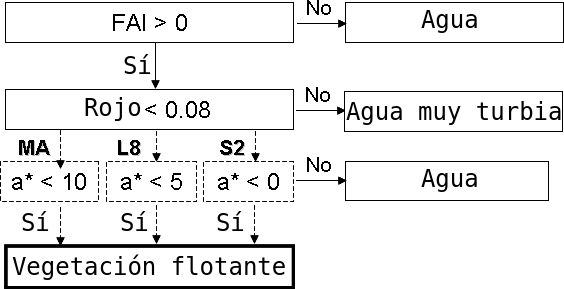
\includegraphics[width=0.6\textwidth]{cam/figures/esquema.png}
        \caption{Diagrama de flujo de la implementación del índice FAIT aquí desarrollado para la detección de vegetación flotante en aguas turbias del Río de la Plata.}
        \label{cam:esquema}
        \end{figure}
    
    \subsection{Impacto de la resolución espacial en la detección de VF}
    \label{cam:s:impacto}
    
        En general, los sensores satelitales de resolución espacial mayor pudieron detectar un área total cubierta por VF más grande y también pudieron resolver características de escala más fina que se perdieron en las imágenes de resolución menor (e.g.  MODIS, 250 m). La capacidad de detección de diferentes sensores de alta resolución se analizó y comparó con las imágenes Aqua/MODIS adquiridas el mismo día. L8 identificó varios parches y filamentos de VF a escala fina el 24 de febrero de 2016 (Figura \ref{cam:FAIT_L8S2}). Teniendo en cuenta la misma subregión en ambas imágenes (cuadrado punteado), el área cubierta por la VF identificada (calculada multiplicando el número de píxeles marcados por la superficie nominal del píxel) para L8(30m) y Aqua/MODIS(250m) fue de $5.8 km^{2}$ y $0.48 km^{2}$, respectivamente. A su vez, S2A capturó varios parches muy pequeños ($0.24 km^{2}$) el 9 de febrero de 2016, mientras que para las imágenes Aqua/MODIS (250 m) del mismo día no se detectó VF (Figura \ref{cam:FAIT_L8S2}). Parte de las diferencias entre las imágenes del mismo día de diferentes sensores se esperan debido a la diferencia en el horario de pasada de los satélites ($\sim 4 hs$), pero principalmente debido a la reducción del contraste espectral causado por la resolución espacial más baja. El ejemplo anterior muestra claramente que si el tamaño de los parches de VF es pequeño en comparación con la resolución espacial del sensor, el área cubierta de VF podría subestimarse o no detectarse en absoluto.


        \begin{figure}
        \centering
        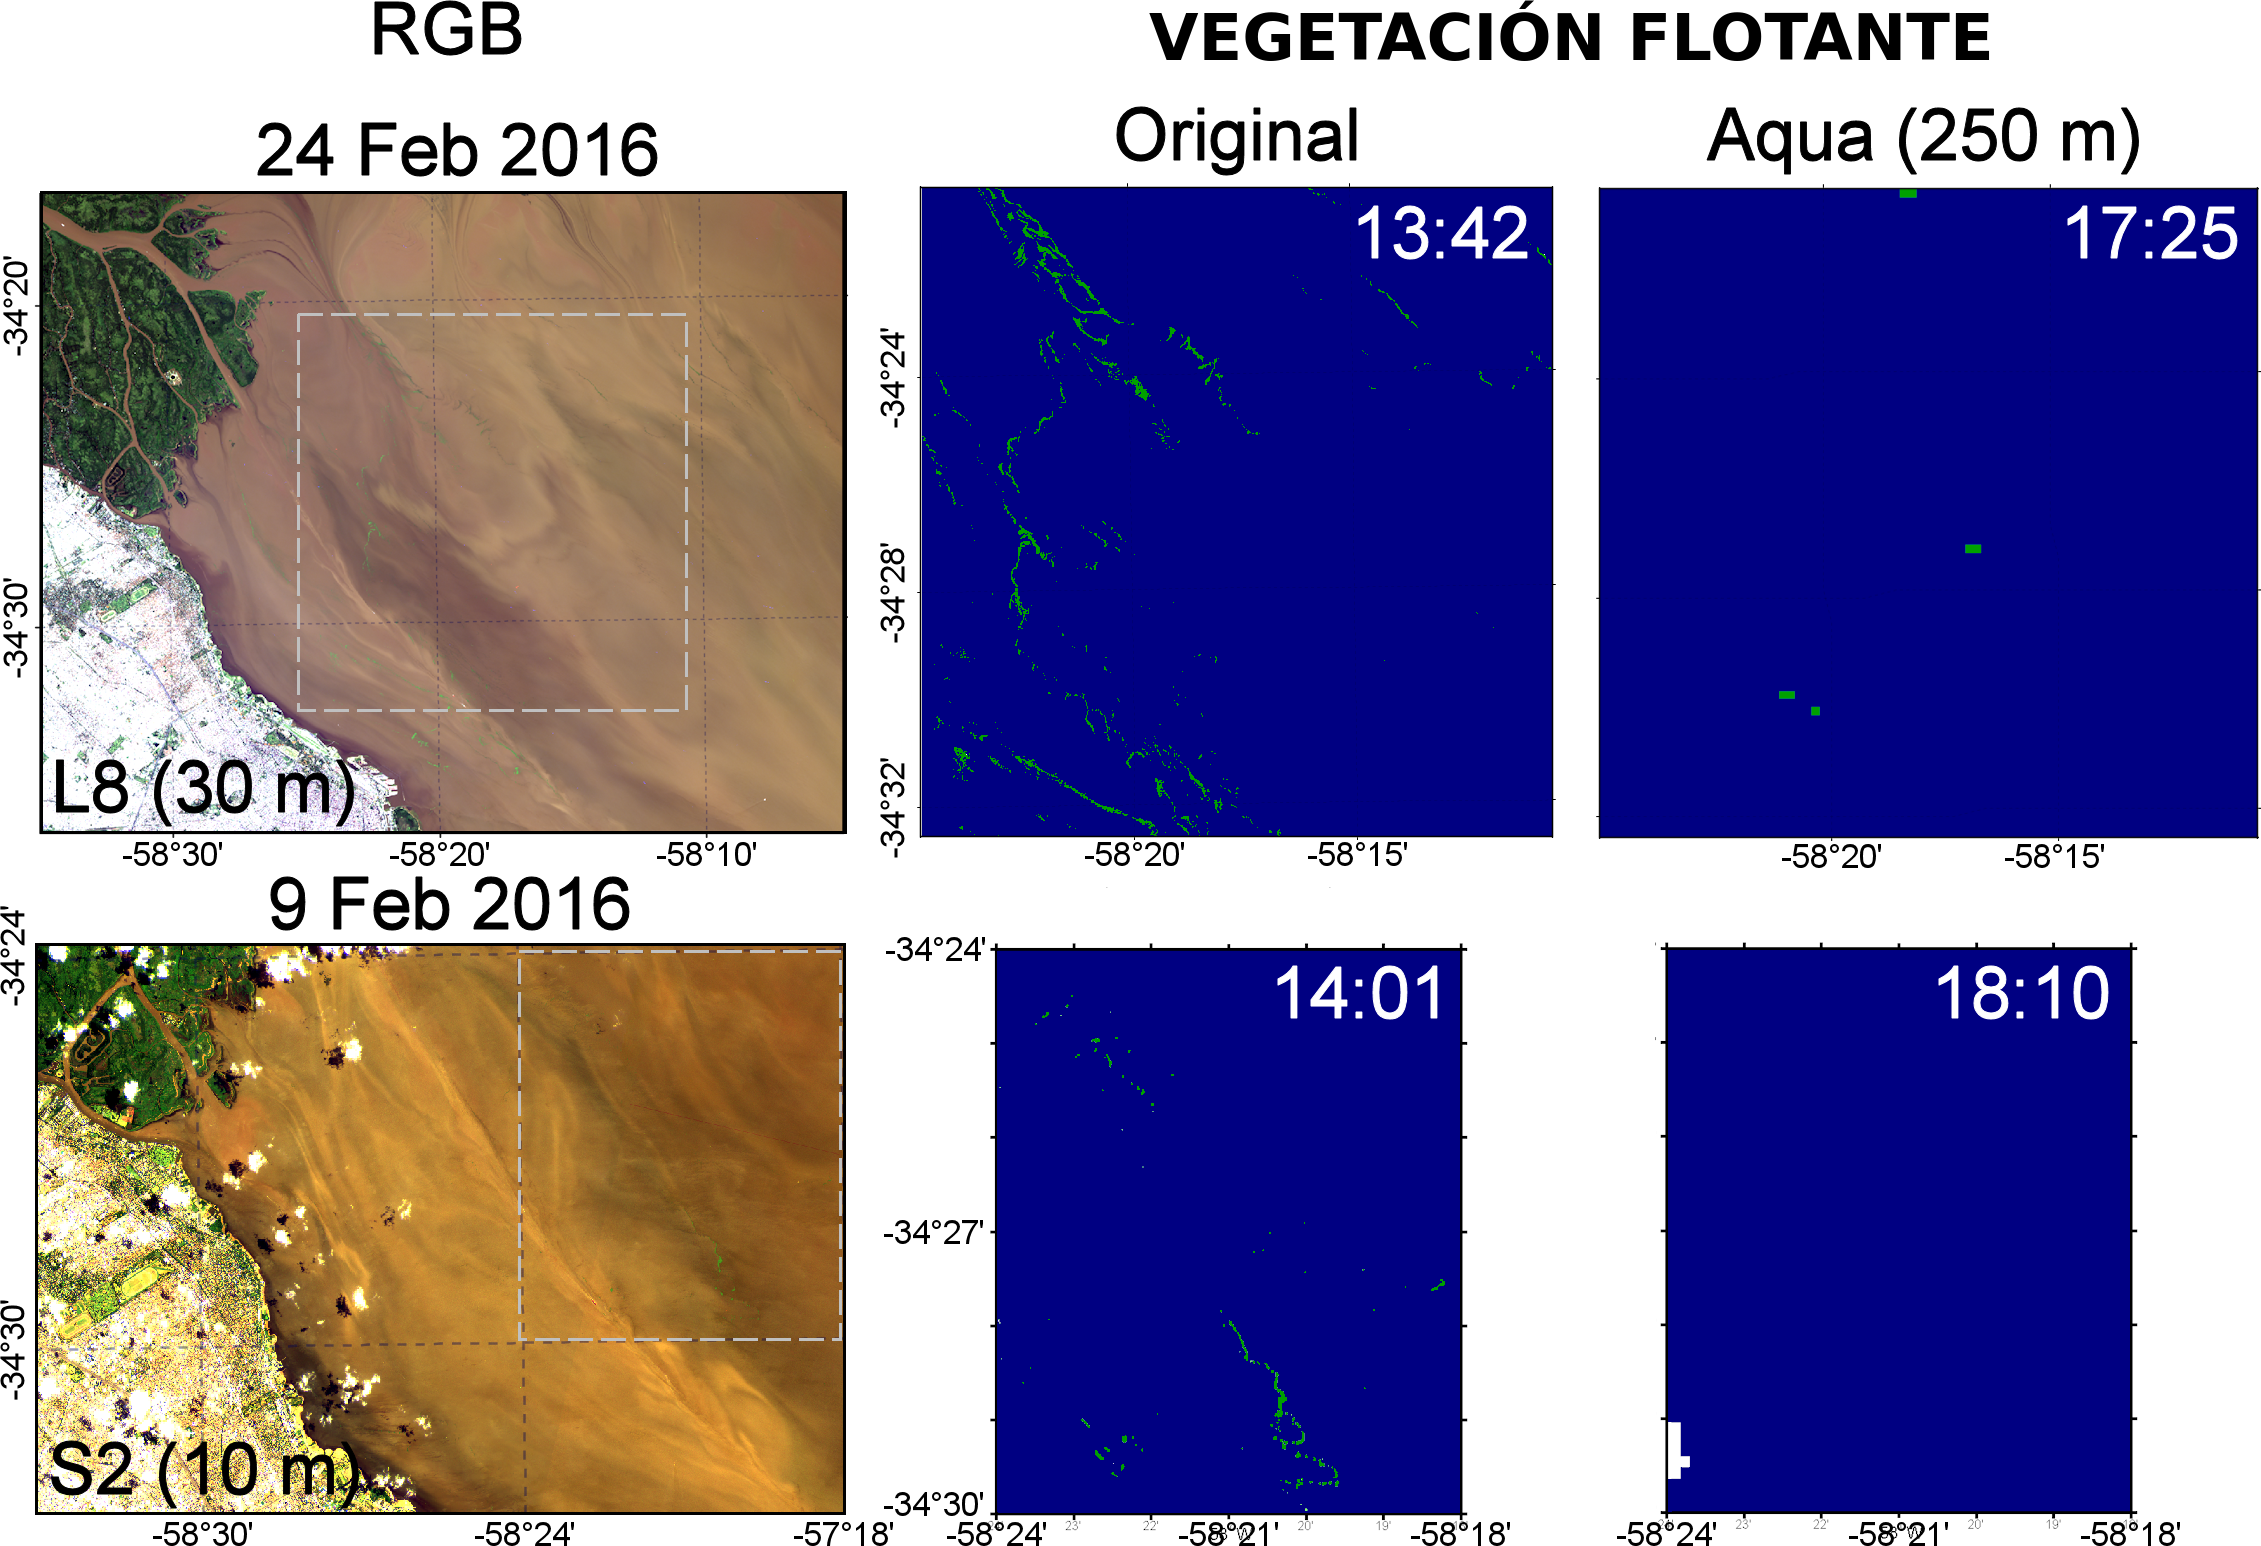
\includegraphics[width=\textwidth]{cam/figures/FAIT_L8S2.png}
        \caption[Composiciones RGB de L8, S2A y Aqua/MODIS e imagen binaria indicando los píxeles con vegetación flotante.]{Composiciones RGB de color de cuasi-verdadero de L8 y S2A (izquierda); píxeles marcados como vegetación flotante para un subconjunto de cada imagen (centro) e imagen Aqua/MODIS del mismo día. También se indica la fecha y hora de adquisición (UTC) de cada imagen.}
        \label{cam:FAIT_L8S2}
        \end{figure}
        
        Para evaluar el impacto de la resolución espacial variable en la capacidad de detección de VF, los datos S2A (10 m) se promediaron espacialmente en cuadrículas más gruesas y los espectros se extrajeron de los datos S2A y se promediaron sobre ventanas espaciales correspondientes a diferentes resoluciones. La Figura \ref{cam:FAIT_RES} muestra datos S2 (9 de febrero de 2016) sobre un parche de VF en la resolución original (10 m) y promediado espacialmente a 30, 300 y 1000 m, junto con los espectros correspondientes. Esta figura muestra la pérdida de contraste espectral como resultado de una resolución espacial reducida, lo que limita la capacidad de los sensores de resoluciones menores para detectar VF. En este caso, la reflectancia correspondiente al píxel de 1000 m de resolución espacial no se clasificaría como cubierta por VF siguiendo el esquema FAIT dado que FAI resultaría negativo (Figura \ref{cam:embarcacion}).
        
        \begin{figure}
        \centering
        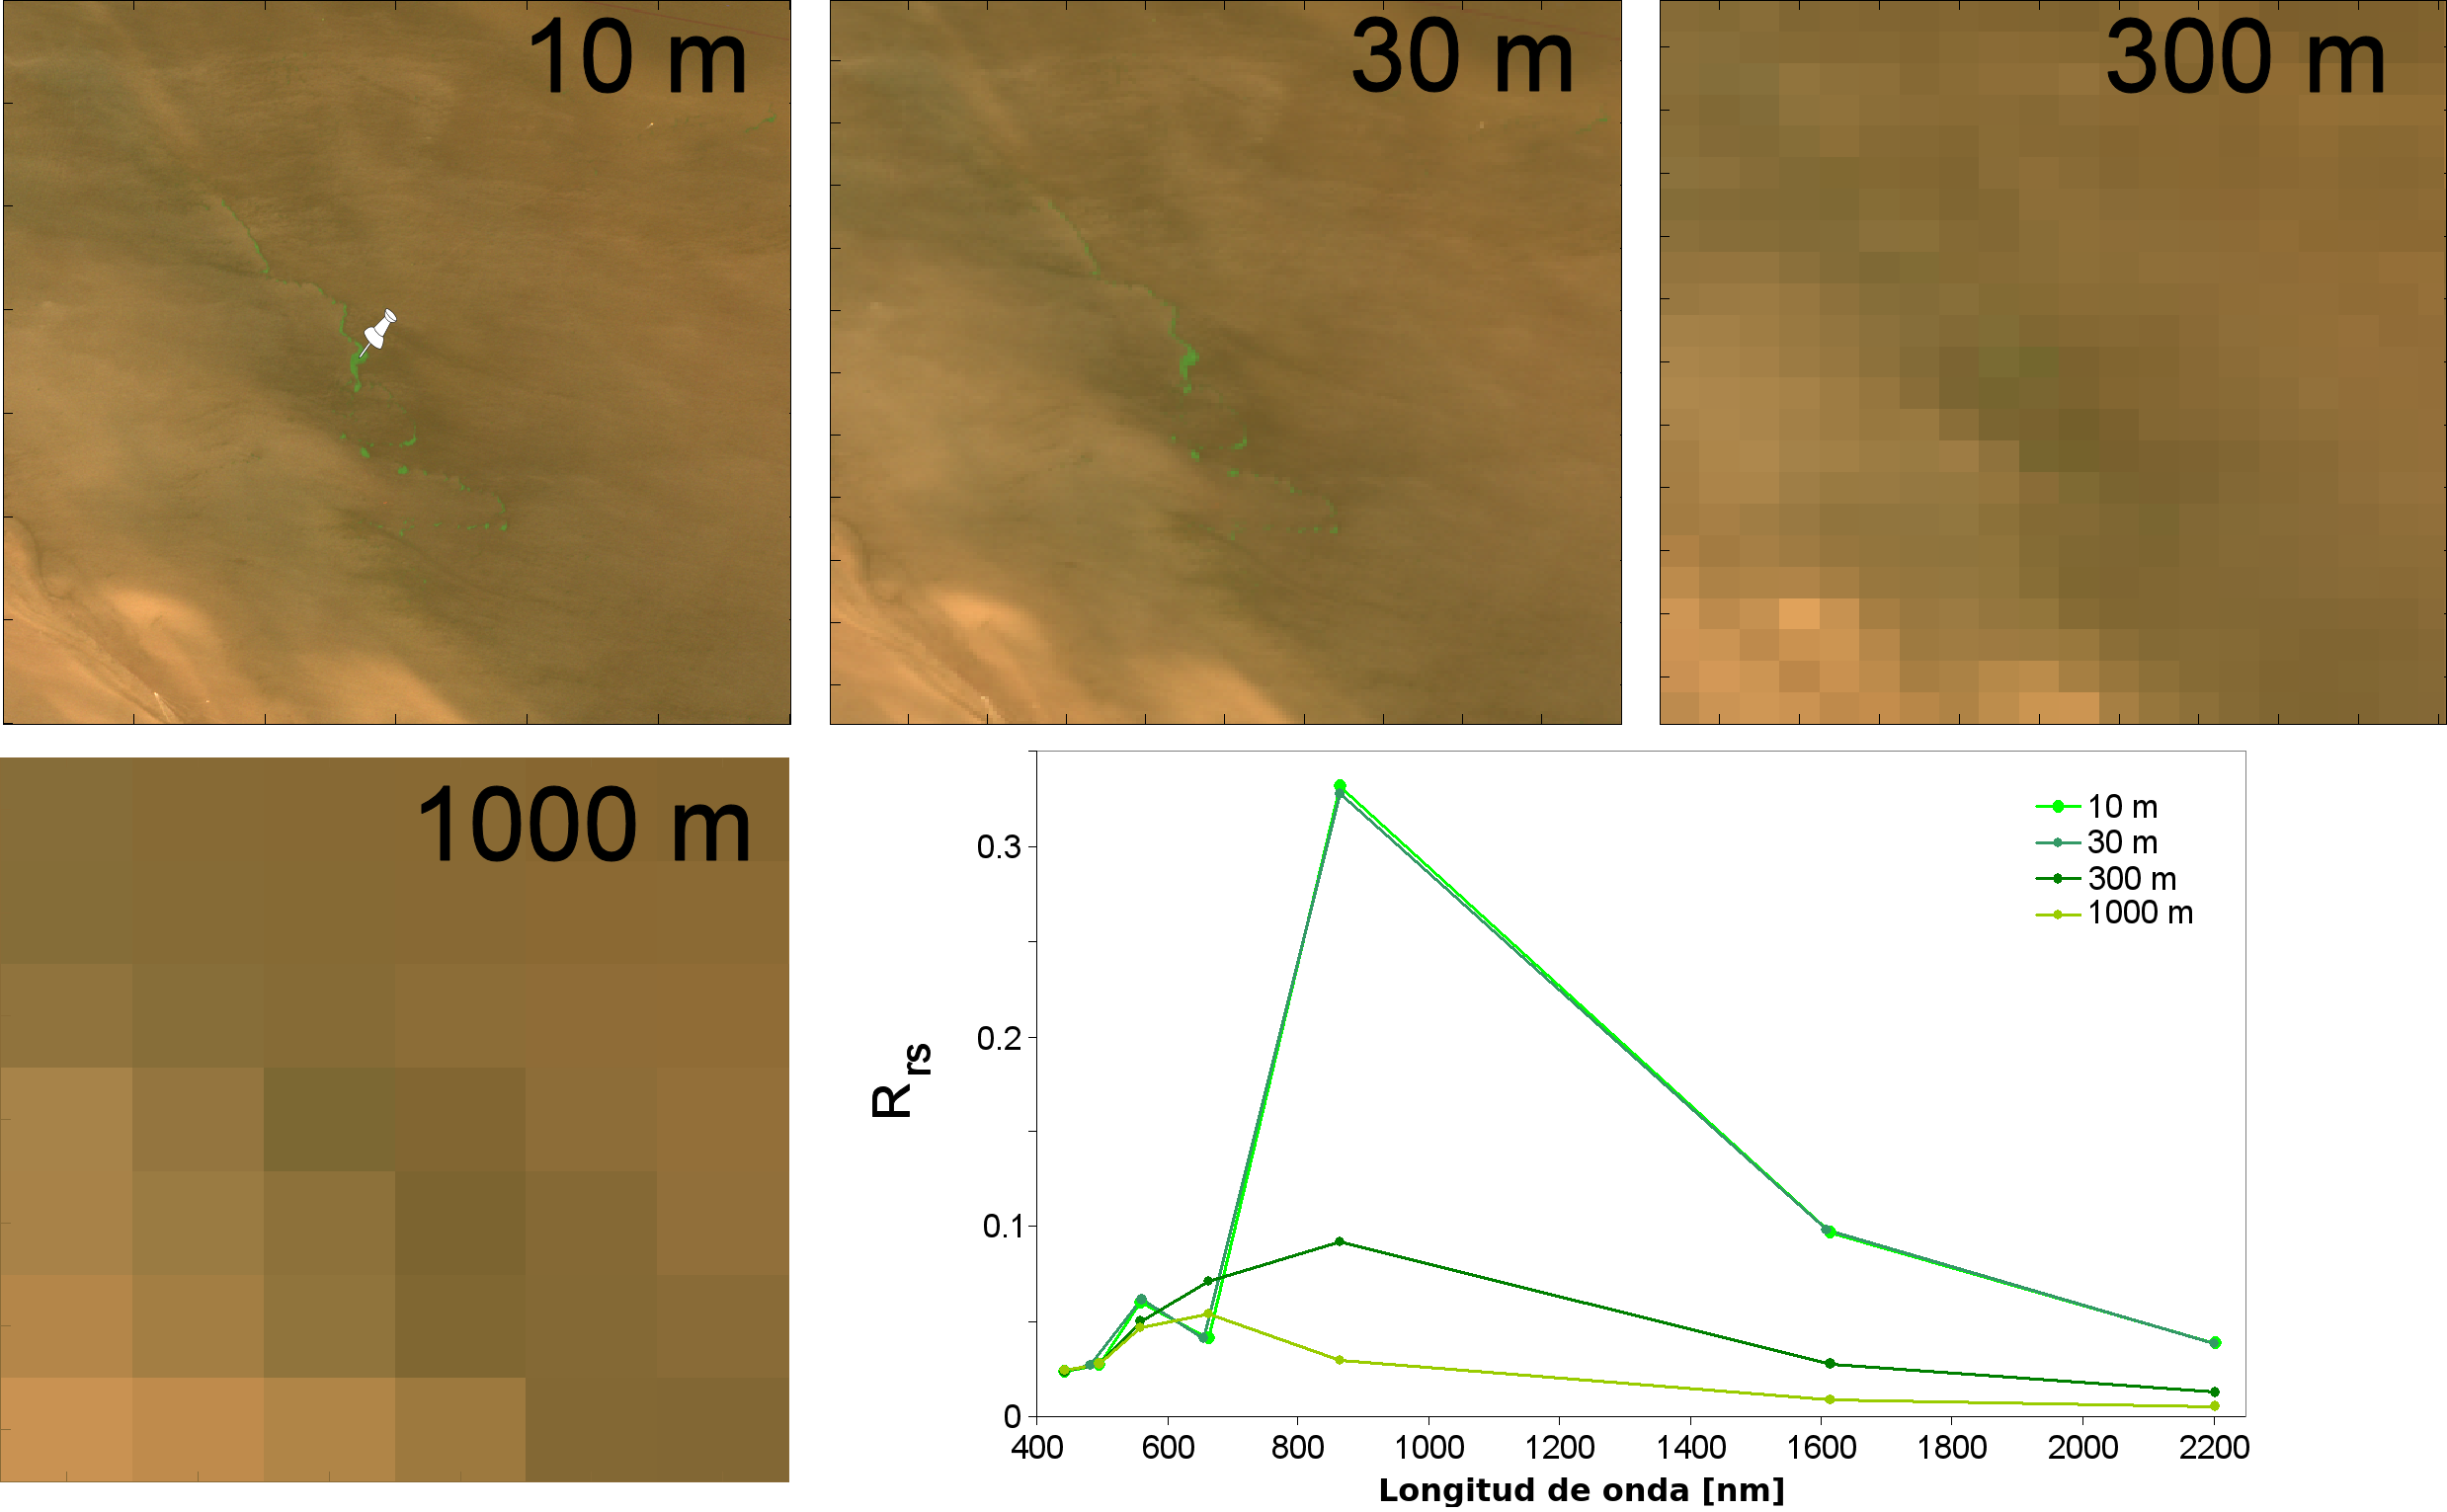
\includegraphics[width=\textwidth]{cam/figures/FAIT_RES.png}
        \caption[Composiciones RGB de imagen S2A sobre un parche de vegetación flotante y efecto de diferentes niveles de degradación espacial.]{Arriba a la izquierda: Composiciones RGB de imagen S2A del 9 de febrero de 2016 sobre un parche de vegetación flotante y suavizados espaciales con píxeles resultantes de 30, 300 y 1000 m. Abajo a la derecha: Espectros correspondientes del píxel verde S2A original y el valor medio aritmético de los cuadros de $3 px \times 3 px$, $29 px \times 29 px$ y $99 px \times 99 px$.}
        \label{cam:FAIT_RES}
        \end{figure}

        Esto está de acuerdo con estudios previos que también sugirieron que la clave principal y el factor limitante para mapear parches de VF es la resolución espacial de los sensores, \cite{hu2009}\cite{cui2012}\cite{xu2015}. La mayor resolución espacial de las bandas L8 y S2 diseñadas para la tierra aumenta su capacidad de detectar VF en comparación con las bandas MODIS-250m, a pesar de su menor sensibilidad radiométrica \cite{hu2009}. Con el fin de estimar el límite de detección espacial del esquema propuesto y su variación con la turbidez del agua, es decir, el porcentaje mínimo de VF en la escala de subpíxeles requerida para ser detectable, se calculó mezclando en diferentes proporciones los miembros finales correspondientes a VF y agua con diferentes turbideces. Similar al análisis realizado por Hu et al. 2015 \cite{hu2015}, se obtuvieron espectros de reflectancias sensadas remótamente (Ec. \ref{int:eq:rrs}) de píxeles simulados ($R_{rs,s}$) utilizando diferentes proporciones ($P_{VF}$, que varían de $0$ a $1$) de los espectros de reflectancia de VF ($R_{rs,VF}$) y agua ($R_{rs,w}$) siguiendo

        
        \begin{equation}
            R_{rs,s} = R_{rs,VF}\times P_{VF} + R_{rs,w} \times (1-P_{VF})
            \label{cam:eq:endmembers}
        \end{equation}
        
        \noindent
        Los miembros de extremo (\textit{endmembers}) se seleccionaron en diferentes imágenes de reflectancia RC de S2 y se muestran en la Figura \ref{cam:endmembers}. Se obtuvo un espectro de VF típico de S2 recolectado el 9 de febrero de 2016 (ver Figura \ref{cam:FAIT_L8S2}) y se obtuvieron cuatro espectros de agua de diferentes imágenes teniendo en cuenta diferentes condiciones:
        
        \begin{enumerate}
            \item \textbf{TW}: Aguas turbias con valores de turbidez típicos de $\sim 120$ FNU en el estuario superior \cite{dogliotti2015} extraído de la misma imagen de donde se tomó el miembro final de VF (9 de febrero de 2016);
            \item \textbf{MT}: Aguas turbias moderadas extraídas del estuario superior donde se espera la máxima turbidez para la región, tal como se describe en Dogliotti et al. 2016 \cite{dogliotti2016} (5 de marzo de 2017);
            \item \textbf{DRG}: Aguas altamente reflectantes y turbias con valores $\sim 600$ FNU (ver Figura \ref{cam:area}), que no se encuentran generalmente en esta región, sino que fueron originadas por una intensa actividad de dragado (17 de agosto de 2016), y
            \item \textbf{XTW}: Aguas extremadamente turbias ($\sim$ 1800 FNU) extraídas de la parte exterior y más turbia del RdP, de la región de Punta Piedras (ver \cite{dogliotti2016}), el 1 de mayo de 2017.
        \end{enumerate}
        
        \begin{figure}
        \centering
        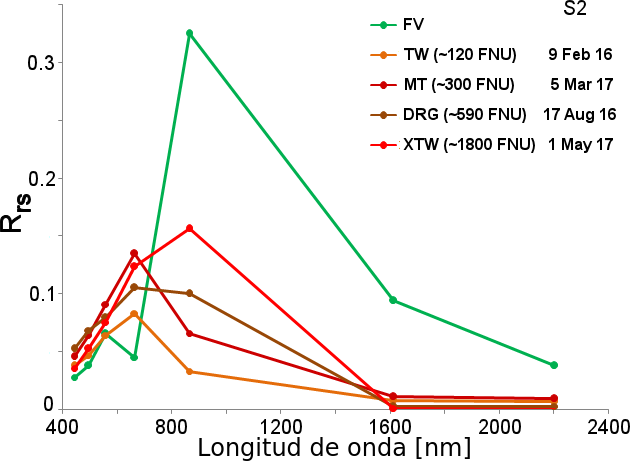
\includegraphics[width=0.7\textwidth]{cam/figures/endmembers.png}
        \caption[Espectros de \textit{endmembers} seleccionados de vegetación flotante y varios tipos de aguas turbias extraídos de diferentes imágenes S2.]{Espectros \textit{puros} (\textit{endmembers}) seleccionados de vegetación flotante (VF), aguas turbias (TW), aguas turbias moderadas (MT), aguas altamente turbias causadas por una intensa actividad de dragado (DRG) y aguas turbias extremas (XTW) extraídas de diferentes imágenes S2 (sólo se muestran las bandas seleccionadas para el algoritmo).}
        \label{cam:endmembers}
        \end{figure}

        Se reporta en el Cuadro \ref{cam:tab:endmembers} el área mínima cubierta requerida dentro de un píxel para ser detectado como contenedor de VF por el esquema FAIT y para activar cada uno de los índices (FAI, Rojo y La$^{*}$b$^{*}$). El análisis mostró que la turbidez tiene un gran efecto sobre la capacidad de detectar VF a partir de imágenes de color del mar. Está claro que el índice FAI no puede usarse sólo para detectar VF dado que la turbidez puede producir falsos positivos que no pueden identificarse \textit{a priori}. En este ejercicio de mezcla de espectros \textit{puros}, el límite de detección es $\sim 10\%$ para aguas turbias típicas y moderadas (Cuadro \ref{cam:tab:endmembers}), pero para aguas muy turbias ($> 500$ FNU) FAI indicaría la presencia de VF incluso si la misma no está presente, lo que confirma la necesidad de condiciones adicionales para evitar falsos positivos. En consecuencia, el límite de detección se debe principalmente al umbral rojo, con un mínimo de $\sim 60 \%$ del área de píxeles que debe cubrirse para las aguas moderadamente y extremadamente turbias y $\sim 40\%$ para la condición particular de la pluma de dragado (DRG) ($\sim 100$ FNU), el \textit{verde} de los píxeles es la condición que determina principalmente el límite de detección ($\sim 28\%$). Esta restricción adicional, aunque más conservadora, evita falsos positivos causados por los bordes de nube y las embarcaciones (Figura \ref{cam:embarcacion}), reduciendo así el límite de detección en comparación con los umbrales FAI y Rojo.

        \begin{table}
        \caption[Porcentaje mínimo de área de píxel ocupada por vegetación flotante necesario para garantizar la detección para diferentes \textit{endmembers} del agua.]{Porcentaje mínimo de área de píxel necesaria para detectar la vegetación flotante (VF, $0 \% W$) para cada condición (índice FAI, umbral rojo, métrica de espacio de color La$^{*}$b$^{*}$) y para el esquema FAIT completo) considerando diferentes \textit{endmembers} del agua ($100 \% W$): aguas turbias (TW), aguas turbias moderadas (MT), aguas altamente turbias debidas a la actividad de dragado (DRG) y aguas extremadamente turbias (XTW). En rojo, procentajes mínimos requeridos de VF nulos para el índice FAI, indicando la necesidad de la aplicación de los índices restantes para evitar falsos positivos.}
        \tiny
        \begin{tabular}{|l|l|l|l|l|l|l|l|l|l|l|}
        \hline
        \textbf{Índice} & \multicolumn{3}{l|}{\textbf{FAI}} & \multicolumn{3}{l|}{\textbf{Rojo}} & \multicolumn{3}{l|}{\textbf{La$^{*}$b$^{*}$}} & \textbf{FAIT}\\ \hline
        \textbf{Fracción} & \textbf{100\%W} & \textbf{0\%W} & \textbf{Min\%} & \textbf{100\%W} & \textbf{0\%W} & \textbf{Min\%} & \textbf{100\%W} & \textbf{0\%W} & \textbf{Min\%} & \textbf{Min\%} \\ \hline
        \textbf{TW}         & -0.0336 & 0.2686 & 11.1                       & 0.0834  & 0.043 & 9.1    & 10.6957 & -26.418       & 28.3   & \textbf{28.3}   \\ \hline
        \textbf{MT}         & -0.0413 & 0.2686 & 13.4                       & 0.1345  & 0.043 & 61.2   & 15.2198 & -26.418       & 51.8   & \textbf{61.2}   \\ \hline
        \textbf{DRG}        & 0.0175  & 0.2686 & {\color[HTML]{FE0000} 0.0} & 0.1053  & 0.043 & 42.3   & 17.1252 & -26.418       & 40.0   & \textbf{42.3}   \\ \hline
        \textbf{XTW}        & 0.0596  & 0.2686 & {\color[HTML]{FE0000} 0.0} & 0.1235  & 0.043 & 55.8   & 30.3149 & -26.418       & 56.2   & \textbf{56.2}   \\ \hline
        \end{tabular}
        \label{cam:tab:endmembers}
        \end{table}

    \subsection{Análisis temporal de la cobertura de vegetación flotante}
    \label{cam:s:temporal}
        Dado el impacto significativo que tuvo este evento en las actividades humanas en la ciudad de Buenos Aires, se definió una región de interés (ROI $\sim 500 km^{2}$) cercana a la misma para evaluar la duración y la cobertura espacial de la invasión de VF (cuadro gris discontinuo en la Figura \ref{cam:area}a). Se procesaron series temporales de imágenes Aqua/MODIS, Landsat-8/OLI y Sentinel-2/MSI para el período 2015 y 2016 con el fin de evaluar el algoritmo durante sendos años con y sin VF (2016 y 2015, respectivamente). Dado el gran tamaño del estuario, los gránulos L8 y S2 lo cubren sólo parcialmente (Figura \ref{cam:area}a). Por lo tanto, se utilizaron los gránulos Path/Row=225/84 de L8 y 21HUB de S2A, y luego de una inspección visual, sólo se seleccionaron imágenes con al menos $10 \%$ de píxeles válidos (no nublados) dentro de la ROI. El número de imágenes analizadas y el área total estimada cubierta por VF durante el período 2015-2016 en la ROI se pueden encontrar en el Cuadro \ref{cam:tab:area} y la distribución temporal de las imágenes en la Figura \ref{cam:area}b (arriba). Dada la resolución temporal reducida y la frecuente presencia de nubes de los sensores de resolución espacial más alta (0.3 y 5.8 $km^{2}$ para S2A y L8, respectivamente, Cuadro \ref{cam:tab:sistemas}) se disponía de menos imágenes y se estimó un área de VF total más pequeña. Se observa que el número reducido de imágenes S2A en 2015 se debió principalmente al hecho de que se lanzó a mediados de junio de 2015 y las imágenes están disponibles sólo desde julio de ese año.


        \begin{figure}
        \centering
        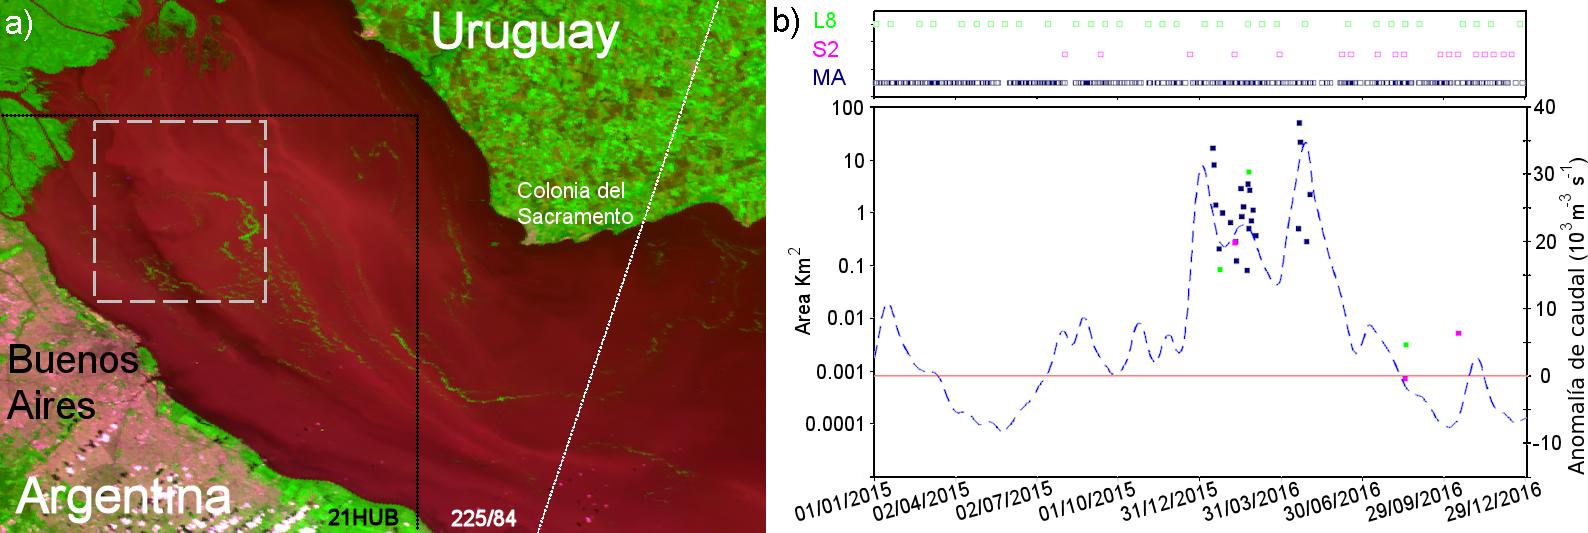
\includegraphics[width=\textwidth]{cam/figures/area.png}
        \caption[Área de vegetación flotante detectada por OLI, MSI-A y Aqua/MODIS para el período de tiempo 2015-2016 y la anomalía de caudal del RdP.]{Composición de color cuasi-verdadero de PROBA-V (R = 650 nm, G = 835 nm, B = 470 nm). a) Imagen (100 m) adquirida el 22 de abril de 2016 que muestra la región de interés (ROI) utilizada para el análisis de cobertura de VF (cuadrado gris discontinuo), área del gránulo 21HUB de S2A (línea negra punteada) y área del gránulo path/row 225/84 de L8 (línea blanca punteada). b) Área de VF (en $km^{2}$) detectada por L8 (verde), S2 (magenta), MA (azul) para el período de tiempo 2015-2016 superpuesto sobre la anomalía de caudal del RdP (línea discontinua de color azul claro). La disponibilidad de imágenes no nubladas para cada sensor se muestra en la parte superior.}
        \label{cam:area}
        \end{figure}
        
        Las primeras y últimas imágenes MODIS que detectaron VF se adquirieron el 15 de enero y el 3 de mayo de 2016, respectivamente. Entre el 8 y el 15 de enero de 2016 no hubo imágenes de la región sin nubes, por lo que no se puede determinar la fecha exacta del cominezo de la invasión de VF. Sin embargo, las primeras observaciones humanas de VF que llegó a la costa de Buenos Aires se realizaron el 16 de enero de 2016 y la llegada de grandes masas no fue continua sino en pulsos después de fuertes lluvias y, por lo tanto, días nublados. Dentro de este período, el caudal de salida del RdP aumentó considerablemente debido a las fuertes lluvias relacionadas con un año de El Niño en fase positiva, \cite{ropewelski1987}\cite{mason2001}.
        % http://www.fao.org/fileadmin/user_upload/emergencies/docs/ElNinoandRainfall.pdf
        Se puede observar claramente en la Figura \ref{cam:area}b que la ocurrencia de un gran área de VF detectada por MODIS coincidió con el aumento de la anomalía del flujo de salida (línea azul discontinua). Desde agosto hasta principios de diciembre de 2016, las imágenes L8 y S2A también detectaron algunos píxeles con VF, pero estos no estaban relacionados con el epsisodio de invasión, sino con vegetación que se desarrolló en una isla temporaria que fue producida por una mayor actividad de dragado durante este período y que se observa claramente en las imágenes S2A RGB (Figura \ref{cam:monticulo}). Este fenómeno implicó una sobreestimación de VF en dichas imágenes y refuerza la necesidad de una máscara de tierra de calidad para poder disponer de estimaciones precisas mediante la implementación del algoritmo.

        
        \begin{table}
        \caption[Área total cubierta por VF estimada a partir del número de píxeles detectados por cada sensor y su resolución espacial para el período 2015-2016 en la región indicada en la Figura \ref{cam:endmembers}.]{Área total cubierta por VF estimada a partir del número de píxeles detectados por cada sensor para el período 2015-2016 en la región indicada en la Figura \ref{cam:endmembers} multiplicada por la resolución espacial nominal correspondiente a cada sensor. También se indica el número de imágenes utilizadas para 2015 (N2015) y 2016 (N2016). *Nótese que Sentinel-2A despegó el 23 de junio de 2015.}
        \begin{tabular}{|l|l|l|l|}
        \hline
        \textbf{Sensor}     & \textbf{Área Total VF [$km^{2}$]} & \textbf{N\_{2015}} & \textbf{N\_{2016}} \\ \hline
        \textbf{Aqua/MODIS} & 114.0                             & 185                & 158                \\ \hline
        \textbf{L8/OLI}     & 5.8                               & 17                 & 15                 \\ \hline
        \textbf{S2A/MSI}    & 0.3                               & 3*                 & 15                 \\ \hline
        \end{tabular}
        \label{cam:tab:area}
        \end{table}

        \begin{figure}
        \centering
        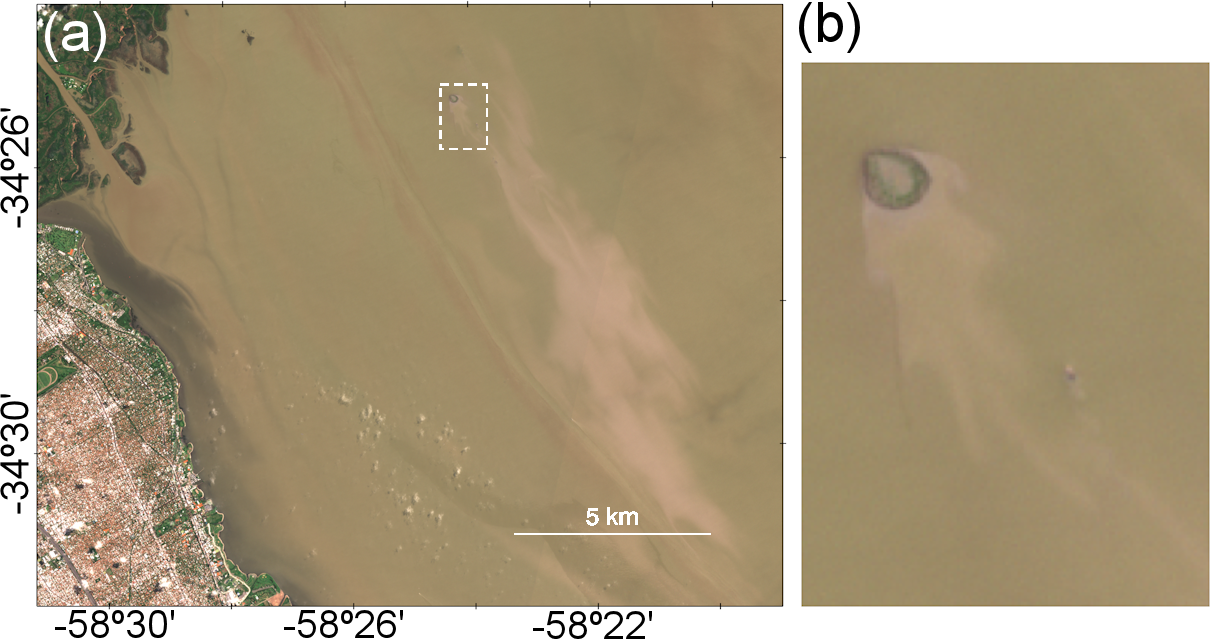
\includegraphics[width=\textwidth]{cam/figures/monticulo.png}
        \caption[Composición RGB de la imagen de Sentinel-2A del 16-OCT-2016 mostrando una pluma turbia y una isla temporaria producidas por sedimentos resuspendidos tras las actividades de dragado.]{Composición RGB de la imagen de Sentinel-2A adquirida el 16 de octubre de 2016. (a) Se ve claramente una pluma de color marrón claro paralela a la línea costera de Buenos Aires producida por sedimentos resuspendidos tras las actividades de dragado; y (b) una ampliación (cuadro punteado en (a)) muestra los detalles de la vegetación desarrollada en la isla temporaria generada por la acumulación de sedimentos durante el dragado.}
        \label{cam:monticulo}
        \end{figure}

\section{Conclusiones}
\label{cam:s:conclusiones}
    En este capítulo se presentó una metodología que permitió identificar y mapear la invasión del jacinto acuático flotante (\textit{Eichhornia crassipes}) en las aguas altamente turbias del RdP que aconteció a partir de enero de 2016. La misma se basa en una combinación del índice FAI (que hace uso de la señal fuerte en la parte NIR del espectro), junto con condiciones adicionales establecidas en la banda roja (para evitar clasificar erróneamente aguas muy turbias) y en las coordenadas de espacio de color La$^{*}$b$^{*}$ (para discriminar la presencia de VF de otros objetos flotantes a partir de la apariencia \textit{verdosa} de los píxeles contenedores de VF). Una de las limitaciones del método presentado es que el FAI no es capaz de distinguir las plantas vasculares acuáticas de la espuma generada por las cianobacterias dada la respuesta similar que tienen en la región NIR como ya se informó \cite{hu2010b} \cite{oyama2015}, lo que produciría falsos positivos de VF. Para el evento específico de 2016 aquí analizado, no se ha reportado floración de cianobacterias en el estuario superior, a pesar de que dichas floraciones  han sido detectadas en diferentes partes de la costa del RdP desde 1982 (\textit{Microcystis spp.} y \textit{Anabaena spp.} son las especies más comunes). En general, se han detectado grandes floraciones de cianobacterias en la costa norte y en la parte exterior del estuario en aguas más claras \cite{dogliotti2016b}. Para poder tener un método global automatizado para diferenciarlos, se necesitan sensores con mayor resolución espectral, por ejemplo, sería útil una banda alrededor de $\sim 620$ nm dado que el pigmento característico presente en las células de cianobacterias llamado ficocianina (PC) tiene un pico de absorción local a esa longitud de onda (Figura \ref{dat:HyperTriOS}). Qi et al. 2014 \cite{qi2014}  han propuesto recientemente un algoritmo que utiliza la banda MERIS 620 nm para estimar las floraciones de PC, en el que tanto las células de cianobacterias como la espuma fueron detectadas y consideradas como floración.
    %
    Por lo tanto, los sistemas multiespectrales existentes que poseen esta banda, como Sentinel-2/MSI, y posibles futuras misiones satelitales hiperespectrales como HyspIRI, proporcionarían información esencial para mejorar la capacidad de mapear VF de manera inequívoca y más precisa sin necesidad de datos de campo. Actualmente, la principal limitación de los datos de Sentinel-2 es la resolución temporal reducida, como se ha señalado en el presente capítulo. Para este evento de 2016, las imágenes diarias MODIS-250m permitieron determinar el período que duró la invasión de VF ($\sim 5$ meses) y hacer una cuantificación aproximada de su extensión. Sin embargo, los sensores de mayor resolución espacial, como Landsat-8 y Sentinel-2, demostraron ser capaces de detectar características de escala más fina y cuantificar mejor la extensión de la VF a pesar de su menor sensibilidad en comparación con las bandas más gruesas de MODIS-250m. Se ha demostrado que la capacidad de detectar VF depende en gran medida de la turbidez del agua, con un límite de detección (mínimo $\%$ del píxel S2-10 m cubierto por VF) de $\sim 30 \%$ para aguas turbias estándar ($\sim 100$ FNU) y $\sim 60 \%$ para aguas de turbideces moderadas a extremas ($> 500$ FNU). Los resultados indican que se necesitan altas resoluciones espaciales y temporales para mejorar la detección y cuantificación de VF, pero el uso sinérgico de varias misiones satelitales disponibles, como en el presente capítulo, también puede proporcionar información útil. Ya se ha logrado una mejora adicional en la resolución temporal con el reciente lanzamiento de Sentinel-2B en marzo de 2017, incrementando la frecuencia de revisión de 10 a 5 días en condiciones sin nubes y hasta 2 ó 3 días si el área de interés está cubierta por pasadas adyacentes.
